\documentclass[
  bibliography=totoc,     % Literatur im Inhaltsverzeichnis
  captions=tableheading,  % Tabellenüberschriften
  titlepage=firstiscover, % Titelseite ist Deckblatt
]{scrartcl}

% Vektoren
\usepackage{esvect}


% Paket float verbessern
\usepackage{scrhack}

% Warnung, falls nochmal kompiliert werden muss
\usepackage[aux]{rerunfilecheck}

% unverzichtbare Mathe-Befehle
\usepackage{amsmath}
% viele Mathe-Symbole
\usepackage{amssymb}
% Erweiterungen für amsmath
\usepackage{mathtools}

% Fonteinstellungen
\usepackage{fontspec}
% Latin Modern Fonts werden automatisch geladen
% Alternativ zum Beispiel:
%\setromanfont{Libertinus Serif}
%\setsansfont{Libertinus Sans}
%\setmonofont{Libertinus Mono}

% Wenn man andere Schriftarten gesetzt hat,
% sollte man das Seiten-Layout neu berechnen lassen
\recalctypearea{}

% deutsche Spracheinstellungen
\usepackage{polyglossia}
\setmainlanguage{german}

% Blindtext
\usepackage{blindtext}

\usepackage[
  math-style=ISO,    % ┐
  bold-style=ISO,    % │
  sans-style=italic, % │ ISO-Standard folgen
  nabla=upright,     % │
  partial=upright,   % ┘
  warnings-off={           % ┐
    mathtools-colon,       % │ unnötige Warnungen ausschalten
    mathtools-overbracket, % │
  },                       % ┘
]{unicode-math}

% traditionelle Fonts für Mathematik
\setmathfont{Latin Modern Math}
% Alternativ zum Beispiel:
%\setmathfont{Libertinus Math}

\setmathfont{XITS Math}[range={scr, bfscr}]
\setmathfont{XITS Math}[range={cal, bfcal}, StylisticSet=1]

% Zahlen und Einheiten
\usepackage[
  locale=DE,                   % deutsche Einstellungen
  separate-uncertainty=true,   % immer Fehler mit \pm
  per-mode=symbol-or-fraction, % / in inline math, fraction in display math
]{siunitx}

% chemische Formeln
\usepackage[
  version=4,
  math-greek=default, % ┐ mit unicode-math zusammenarbeiten
  text-greek=default, % ┘
]{mhchem}

% richtige Anführungszeichen
\usepackage[autostyle]{csquotes}

% schöne Brüche im Text
\usepackage{xfrac}
\usepackage{nicefrac}

% Standardplatzierung für Floats einstellen
\usepackage{float}
\floatplacement{figure}{htbp}
\floatplacement{table}{htbp}

% Floats innerhalb einer Section halten
\usepackage[
  section, % Floats innerhalb der Section halten
  below,   % unterhalb der Section aber auf der selben Seite ist ok
]{placeins}

% Seite drehen für breite Tabellen: landscape Umgebung
\usepackage{pdflscape}

% Captions schöner machen.
\usepackage[
  labelfont=bf,        % Tabelle x: Abbildung y: ist jetzt fett
  font=small,          % Schrift etwas kleiner als Dokument
  width=0.9\textwidth, % maximale Breite einer Caption schmaler
]{caption}
% subfigure, subtable, subref
\usepackage{subcaption}

% Grafiken können eingebunden werden
\usepackage{graphicx}
% größere Variation von Dateinamen möglich
\usepackage{grffile}

% schöne Tabellen
\usepackage{booktabs}

% Verbesserungen am Schriftbild
\usepackage{microtype}

% Literaturverzeichnis
\usepackage[
  backend=biber,
]{biblatex}
% Quellendatenbank
\addbibresource{lit.bib}
\addbibresource{programme.bib}

% Hyperlinks im Dokument
\usepackage[
  unicode,        % Unicode in PDF-Attributen erlauben
  pdfusetitle,    % Titel, Autoren und Datum als PDF-Attribute
  pdfcreator={},  % ┐ PDF-Attribute säubern
  pdfproducer={}, % ┘
]{hyperref}
% erweiterte Bookmarks im PDF
\usepackage{bookmark}

% Trennung von Wörtern mit Strichen
\usepackage[shortcuts]{extdash}
%Erlaubt Einfügen von PDF-Dateien
\usepackage{pdfpages}
\author{%
  Lars Kolk\\%
  \href{mailto:lars.kolk@tu-dortmund.de}{lars.kolk@tu-dortmund.de}%
  \texorpdfstring{\and}{,}%
  Julia Sobolewski\\%
  \href{mailto:julia.sobolewski@tu-dortmund.de}{julia.sobolewski@tu-dortmund.de}%
  \texorpdfstring{\and}{,}%
  Jannine Salewski\\%
  \href{mailto:Jannine.salewski@tu-dortmund.de}{jannine.salewski@tu-dortmund.de}%
}
\publishers{TU Dortmund – Fakultät Physik}

\usepackage{longtable}
\usepackage{wrapfig}
\usepackage{ dsfont }
\usepackage{tcolorbox}
\subject{SMD-Abgabe}
\title{1. Übungsblatt}
\date{%
  Abgabe: 25.10.2018
}

\begin{document}
  \setlength{\parindent}{0em}
  \maketitle
  \thispagestyle{empty}
  \newpage
  \tableofcontents
  \newpage

  \newenvironment{console1}[1]
  {\begin{center}
  \begin{minipage}[t]{0.99\linewidth}
  \begin{tcolorbox}[colback=gray!5,colframe=black!40!black,title= Ausgabe des Programms: #1 ]
    }
    {
  \end{tcolorbox}
  \end{minipage}
  \end{center}
  }

\input{Aufgabe06/aufgabe06.tex}
%\section{Aufgabe 2}
\subsection{Teilaufgabe a}
Die Gleichung
\begin{equation}
  \frac{d \sigma}{d \Omega}=\frac{\alpha ^2}{s} \cdot \left(\frac{2+\sin^2{\theta}}{1-\beta^2 \cdot \cos^2{\theta}} \right)
\end{equation}
mit
\begin{align*}
  s=\left( 2E_e\right)^2 \\
  \beta=\sqrt{1-\gamma^{-2}} \\
  \gamma=\frac{E_e}{m_e} \\
  m_e= \SI{511}{keV}
\end{align*}
ist numerisch nicht stabil. Dies lässt sich mit der Folge der vielen Operationen begründen. \\
Außerdem lässt sich in der ausgeschriebenden Form
\begin{equation}
  \frac{d \sigma}{d \Omega}=\frac{\alpha ^2}{4E^2_{e}} \cdot \left(\frac{2+\sin^2{\theta}}{1-\left(1-\frac{m_{e}}{E_{2}} \right) \cdot \cos^2{\theta}} \right)
\end{equation}
sehen, dass die Gleichung für den Fall $\theta = n \cdot \pi$, $n \in \mathbb{Z}$ besonders instabil ist , da
$\cos^2{\pm \pi}=1$ gilt und somit im Nenner  zwei gleichgroße Zahlen voneinander subtrahiert werden.
Zusätzlich findet im Fall $E_e=\SI{50}{GeV}$ eine Division durch eine kleine Zahl statt $\left( {\frac{m_{e}}{E_{2}}}^2 \ll 1 \right)$, womit die Gleichung numerisch instabil ist.


\subsection{Teilaufgabe b} \label{sec:2b}

\begin{align}
  \frac{d \sigma}{d \Omega} &= \frac{\alpha ^2}{s} \cdot \left(\frac{2+\sin^2{\theta}}{1-\beta^2 \cdot \cos^2{\theta}} \right) \\
  &=\frac{\alpha ^2}{s} \cdot \left(\frac{2+\sin^2{\theta}}{1-\beta^2 + \beta^2 \cdot \sin^2{\theta}} \right) \\
  &=\frac{\alpha ^2}{s} \cdot \left(\frac{2+\sin^2{\theta}}{\gamma^{-2} + \left(1-\gamma^{-2} \right) \cdot \sin^2{\theta}} \right) \\
  &=\frac{\alpha ^2}{s} \cdot \left(\frac{2+\sin^2{\theta}}{\gamma^{-2} \cdot \left(1-\sin^{2}{\theta} \right) + \sin^2{\theta}} \right) \\
  &=\frac{\alpha ^2}{s} \cdot \left(\frac{2+\sin^2{\theta}}{\gamma^{-2} \cdot \cos^2{\theta} + \sin^2{\theta}} \right)  \label{eqn:dwqsb}\\
\end{align}
Das Ergebnis ist numerisch stabiler, da die Substraktion zwei gleich großer Zahlen im Nenner aufgrund der Addition von zwei quadratischen Funktionen nicht mehr auftreten kann.

\subsection{Teilaufgabe c}
\begin{figure}[H]
  \centering
  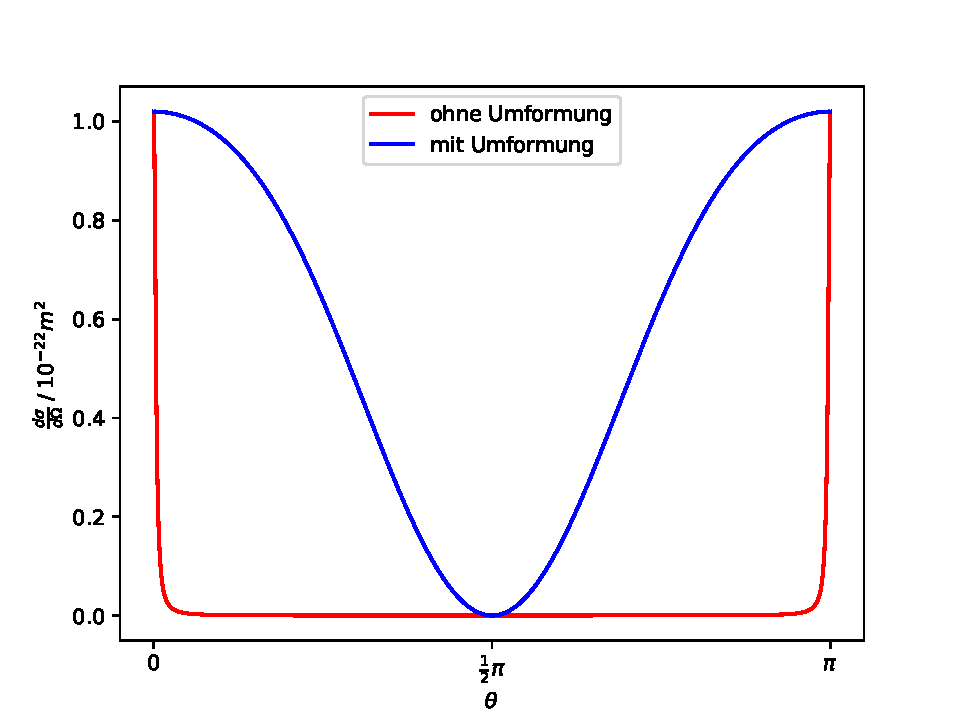
\includegraphics[width=\textwidth]{Aufgabe02/diffquerschnitt.pdf}
  \caption{Darstellung des differentiellen Wirkungsquerschnitts, mit und ohne die Umformung aus \ref{sec:2b} }
  \label{fig:2b}
\end{figure}
Wie in \ref{fig:2b} zu sehen ist, hebt sich die Kurve, die mit der Gleichung aus \eqref{eqn:dwqsb} berechnet wurde, deutlich von der anderen ab.
Statt einem Plateau ist nun eine (grob) parabelförmige Funktion zu sehen, woraus sich schließen lässt, dass dass die neue Funktion \eqref{eqn:dwqsb} numerisch stabiler ist.

\subsection{Teilaufgabe d} \label{sec:2d}
Die Konditionszahl ist definiert durch
\begin{equation}
  k=\mid \frac{f'(x)}{f(x)} \cdot x \mid
\end{equation}
\begin{align}
  f(\theta) &= \frac{\alpha ^2}{s} \cdot \left(\frac{2+\sin^2{\theta}}{1-\beta^2 \cdot \cos^2{\theta}} \right) \\
  f'(\theta) &= -\frac{a^2}{s} \cdot \frac{\cos{\theta} \sin{\theta} \cdot \left(3b^2-1 \right)}{\left (b^2\cos^2{\theta}-1 \right)^2} \\
  \rightarrow k &=  \frac{|\left( 3b^2-1\right) \theta \cdot \sin {\left(2 \theta \right)|}}{| \left(\sin^2{\theta}+2 \right) \cdot \left(\beta^2 \cdot \cos^2{\theta}-1 \right )| } \mid
\end{align}

\subsection{Teilaufgabe d}
\begin{figure}[H]
  \centering
  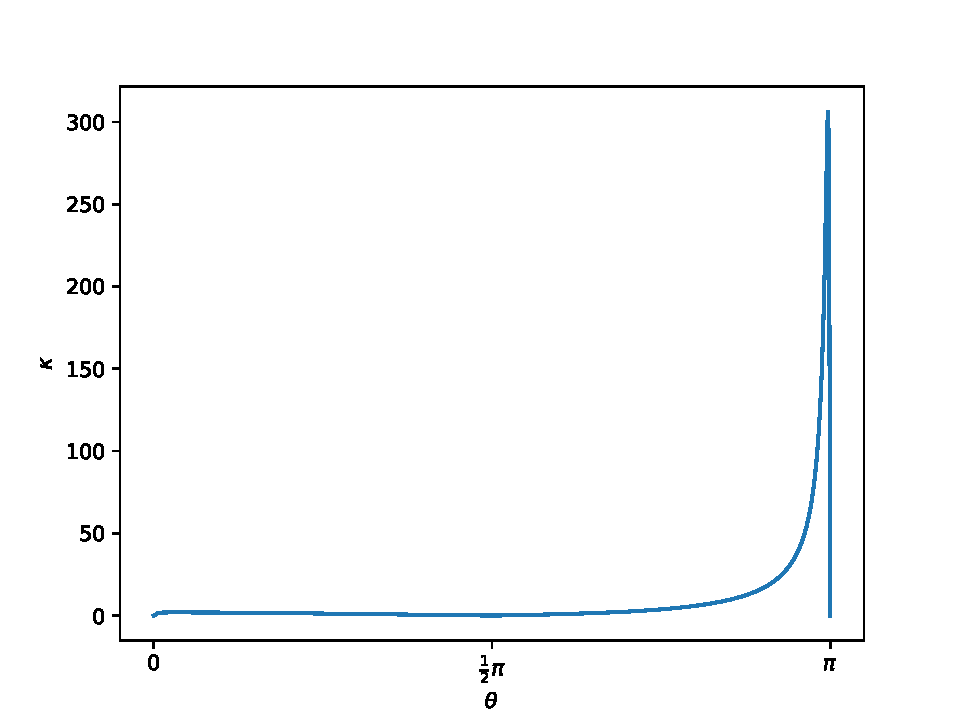
\includegraphics[width=\textwidth]{Aufgabe02/Konditionszahl.pdf}
  \caption{Darstellung der Konditionszahl k aus  \ref{sec:2d} }
  \label{fig:2d}
\end{figure}
Wie in Abbildung \ref{fig:2d} zu sehen ist, ist das Problem gut für $0<x<\pi$ konditioniert.

%\input{Text/Auswertung.tex}
%\paragraph{Aufgabe 4}

\subparagraph{a)}

$P\left(W_\text{rot}+W_\text{blau}=9\right) \: = \: \SI{11,11}{\%}$

\subparagraph{b)}

$P\left(W_\text{rot}+W_\text{blau} \geq 9\right) \: = \: \SI{27,78}{\%}$

\subparagraph{c)}

$P\left(W_\text{rot}=4, W_\text{blau}=5\right \vee W_\text{rot}=5, W_\text{blau}=4) \: \geq \: \SI{5,56}{\%}$

\subparagraph{d)}

$P\left(W_\text{rot}=4, W_\text{blau}=5\right) \: \geq \: \SI{2,78}{\%}$

\subparagraph{e)}

$P\left(W_\text{rot}+W_\text{blau}=9 | W_\text{rot}=4\right) \: = \: \SI{16,67}{\%}$

\subparagraph{f)}

$P\left(W_\text{rot}+W_\text{blau} \geq 9 | W_\text{rot}=4\right) \: = \: \SI{33,33}{\%}$

\subparagraph{g)}

$P\left(W_\text{rot}=4, W_\text{blau}=5\right) \: \geq \: \SI{16,67}{\%}$

%\printbibliography{}


\end{document}
